\documentclass[crop,tikz]{standalone}% 'crop' is the default for v1.0, before it was 'preview'
\usetikzlibrary{arrows.meta}
%\usetikzlibrary{...}% tikz package already loaded by 'tikz' option

\usepackage{bm}
\usepackage{xcolor}
\begin{document}
	
	\definecolor{x1}{HTML}{E64B35}
	\definecolor{x2}{HTML}{4DBBD5}
	\definecolor{x3}{HTML}{3C5488}
	\definecolor{x4}{HTML}{00A087}
	\begin{tikzpicture}[
		my node/.style={circle, black, fill = black!50!white, minimum size=40pt, inner sep=0pt, align = center, scale = 1.1},
		my arrow/.style={-Triangle}
		]
		% Causal Structure
		\node[scale = 1.8] at (1.25, 1.3) {\textbf{Causal structure}};
		\node[my node, fill = x1] (X1) at (0,0) {$\bm{X_1}$\\\textbf{cat.}};
		\node[my node, fill = x2] (X2) at (2.5,0) {$\bm{X_2}$\\\textbf{cont.}};
		\node[my node, fill = x3] (X4) at (0,-2.5) {$\bm{X_4}$\\\textbf{cont.}};
		\node[my node, fill = x4] (X3) at (2.5,-2.5) {$\bm{X_3}$\\\textbf{cat.}};
		\node[my node] (Y) at (1.25,-4.5) {$\bm{Y}$};
		
		\draw[my arrow] (X1) -- (X4);
		\draw[my arrow] (X2) -- (X3);
		\draw[my arrow] (X4) -- (Y);
		\draw[my arrow] (X3) -- (Y);
		
		% Show legend
		\node at (1.25, -7.5) {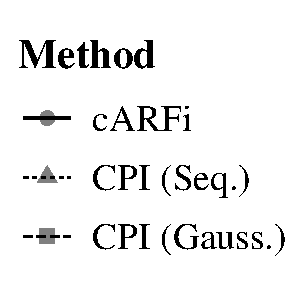
\includegraphics[scale = 0.85]{figures/tmp_plots/legend_mixed_data.pdf}};
		
		% Show plot
		\node at (-9.5, -4.5) {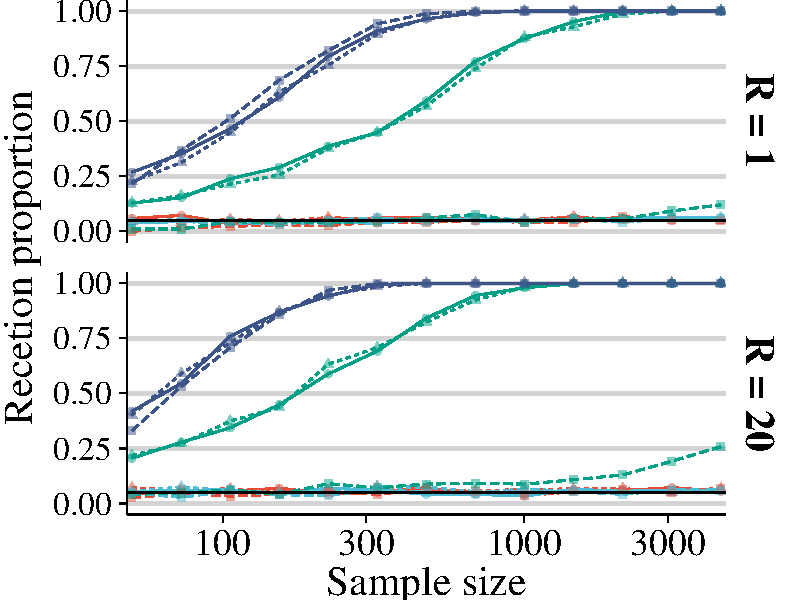
\includegraphics[scale = 1.25]{figures/tmp_plots/plot_mixed_data.pdf}};
	\end{tikzpicture}
\end{document}